\subsection{解释器模式(Interpreter)}

解释器模式是一种行为型设计模式,它提供了一种方法,通过定义一组语言文法规则并使用这些规则来解释语言中的句子,从而可以实现对语言的解释执行。

解释器模式的实现通常包括以下几个部分:
\begin{enumerate}
    \item 定义语言文法规则:首先,我们需要根据需求定义语言的文法规则,并将其表示为一组符号、终结符和非终结符的集合。
    \item 建立抽象语法树:接下来,我们需要使用定义的文法规则来解析语言中的句子,并将其表示为一棵抽象语法树。
    \item 定义解释器:最后,我们需要定义一个解释器,它可以接收一棵抽象语法树作为输入,并根据语言的文法规则来执行对应的操作。
\end{enumerate}

解释器模式的实现需要结合文法规则和语言知识,需要比较细致的设计和实现。使用解释器模式可以有以下几个优点:

\begin{enumerate}
    \item 可以将语言文法规则与语言解释器的实现分离,从而更加灵活地支持对语言的扩展和修改。
    \item 可以通过构建抽象语法树来实现对语言的解释执行,从而使得语言的解释更加高效。
    \item 可以在不改变原有类的情况下为语言的解释器添加额外的功能,例如语法检查、性能监控等。
    \item 可以通过定义统一的抽象语法树来统一语言解释器的实现,从而更加方便地实现多语言支持。
\end{enumerate}

\subsubsection{解释器模式在项目中的应用}

\begin{figure}[h]
    \centering
    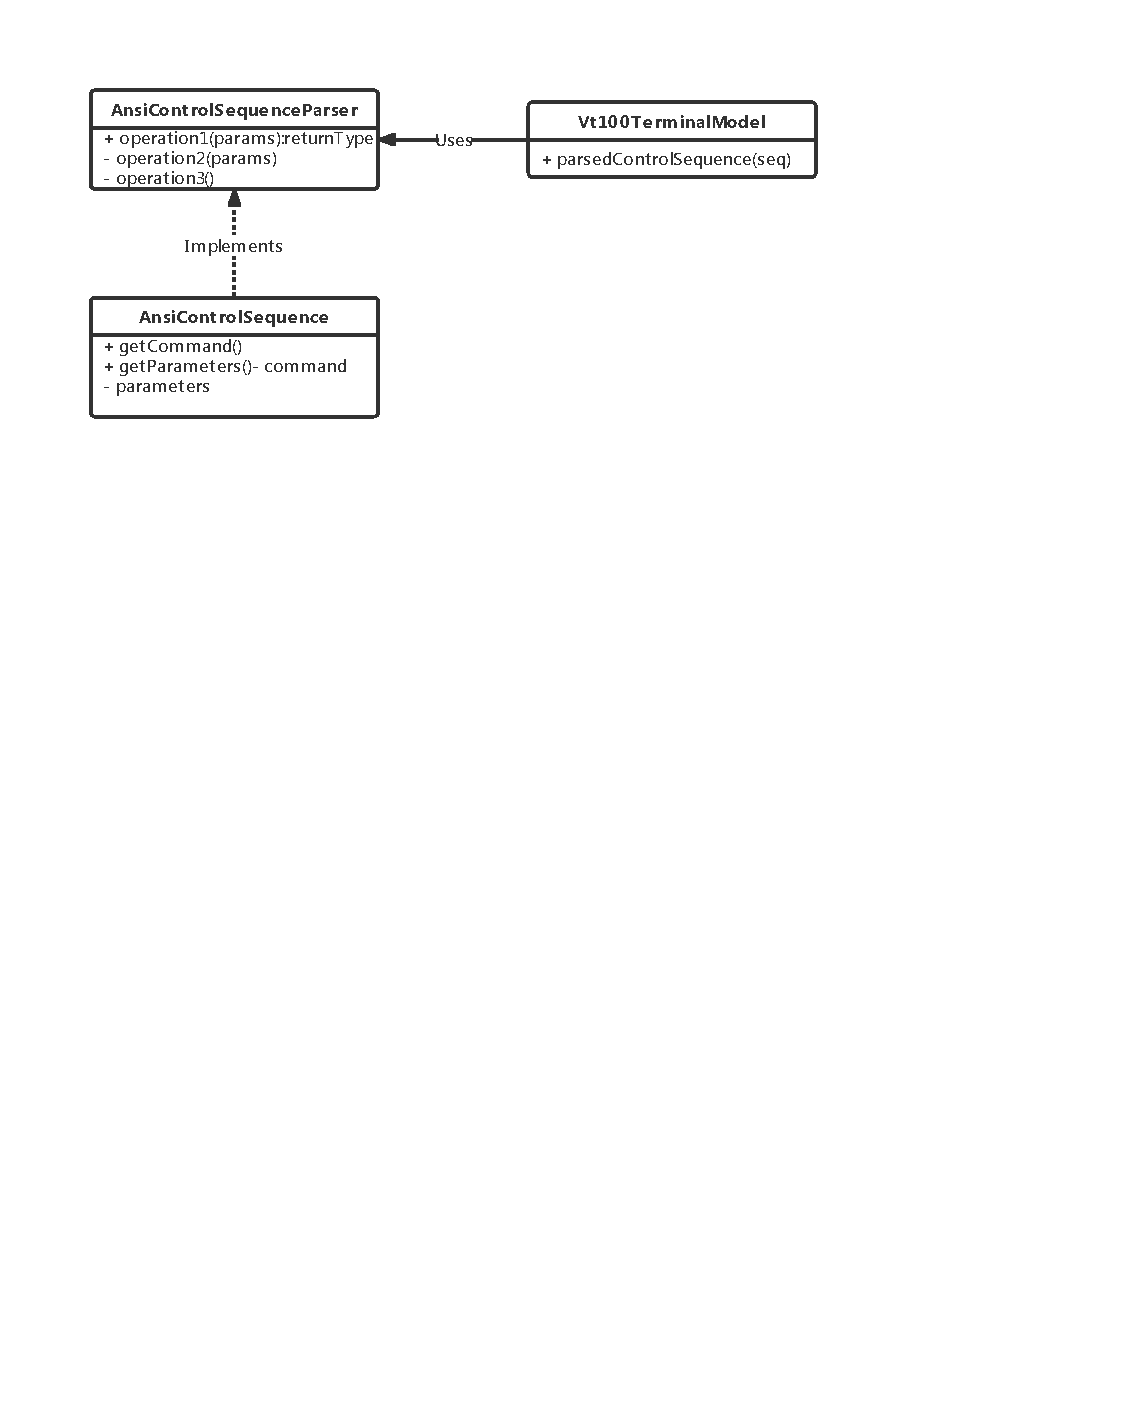
\includegraphics[width=0.9\textwidth]{figures/Interpreter.pdf}
    \caption{解释器模式在 Slow6502 中的类图}
\end{figure}

在我们的项目中,解释器模式主要用于将总线上流动的数据解析为终端外设的 Ansi Control Sequence,解析后的 Ansi Control Sequence 为一串命令,供 VT100 终端使用。这里解释器的语言文法规则较为简洁,即 Ansi Control Sequence 的文法。
